\documentclass[twoside]{book}

% Packages required by doxygen
\usepackage{fixltx2e}
\usepackage{calc}
\usepackage{doxygen}
\usepackage[export]{adjustbox} % also loads graphicx
\usepackage{graphicx}
\usepackage[utf8]{inputenc}
\usepackage{makeidx}
\usepackage{multicol}
\usepackage{multirow}
\PassOptionsToPackage{warn}{textcomp}
\usepackage{textcomp}
\usepackage[nointegrals]{wasysym}
\usepackage[table]{xcolor}

% Font selection
\usepackage[T1]{fontenc}
\usepackage[scaled=.90]{helvet}
\usepackage{courier}
\usepackage{amssymb}
\usepackage{sectsty}
\renewcommand{\familydefault}{\sfdefault}
\allsectionsfont{%
  \fontseries{bc}\selectfont%
  \color{darkgray}%
}
\renewcommand{\DoxyLabelFont}{%
  \fontseries{bc}\selectfont%
  \color{darkgray}%
}
\newcommand{\+}{\discretionary{\mbox{\scriptsize$\hookleftarrow$}}{}{}}

% Page & text layout
\usepackage{geometry}
\geometry{%
  a4paper,%
  top=2.5cm,%
  bottom=2.5cm,%
  left=2.5cm,%
  right=2.5cm%
}
\tolerance=750
\hfuzz=15pt
\hbadness=750
\setlength{\emergencystretch}{15pt}
\setlength{\parindent}{0cm}
\setlength{\parskip}{3ex plus 2ex minus 2ex}
\makeatletter
\renewcommand{\paragraph}{%
  \@startsection{paragraph}{4}{0ex}{-1.0ex}{1.0ex}{%
    \normalfont\normalsize\bfseries\SS@parafont%
  }%
}
\renewcommand{\subparagraph}{%
  \@startsection{subparagraph}{5}{0ex}{-1.0ex}{1.0ex}{%
    \normalfont\normalsize\bfseries\SS@subparafont%
  }%
}
\makeatother

% Headers & footers
\usepackage{fancyhdr}
\pagestyle{fancyplain}
\fancyhead[LE]{\fancyplain{}{\bfseries\thepage}}
\fancyhead[CE]{\fancyplain{}{}}
\fancyhead[RE]{\fancyplain{}{\bfseries\leftmark}}
\fancyhead[LO]{\fancyplain{}{\bfseries\rightmark}}
\fancyhead[CO]{\fancyplain{}{}}
\fancyhead[RO]{\fancyplain{}{\bfseries\thepage}}
\fancyfoot[LE]{\fancyplain{}{}}
\fancyfoot[CE]{\fancyplain{}{}}
\fancyfoot[RE]{\fancyplain{}{\bfseries\scriptsize Generated by Doxygen }}
\fancyfoot[LO]{\fancyplain{}{\bfseries\scriptsize Generated by Doxygen }}
\fancyfoot[CO]{\fancyplain{}{}}
\fancyfoot[RO]{\fancyplain{}{}}
\renewcommand{\footrulewidth}{0.4pt}
\renewcommand{\chaptermark}[1]{%
  \markboth{#1}{}%
}
\renewcommand{\sectionmark}[1]{%
  \markright{\thesection\ #1}%
}

% Indices & bibliography
\usepackage{natbib}
\usepackage[titles]{tocloft}
\setcounter{tocdepth}{3}
\setcounter{secnumdepth}{5}
\makeindex

% Hyperlinks (required, but should be loaded last)
\usepackage{ifpdf}
\ifpdf
  \usepackage[pdftex,pagebackref=true]{hyperref}
\else
  \usepackage[ps2pdf,pagebackref=true]{hyperref}
\fi
\hypersetup{%
  colorlinks=true,%
  linkcolor=blue,%
  citecolor=blue,%
  unicode%
}

% Custom commands
\newcommand{\clearemptydoublepage}{%
  \newpage{\pagestyle{empty}\cleardoublepage}%
}

\usepackage{caption}
\captionsetup{labelsep=space,justification=centering,font={bf},singlelinecheck=off,skip=4pt,position=top}

%===== C O N T E N T S =====

\begin{document}

% Titlepage & ToC
\hypersetup{pageanchor=false,
             bookmarksnumbered=true,
             pdfencoding=unicode
            }
\pagenumbering{roman}
\begin{titlepage}
\vspace*{7cm}
\begin{center}%
{\Large My Project }\\
\vspace*{1cm}
{\large Generated by Doxygen 1.8.11}\\
\end{center}
\end{titlepage}
\clearemptydoublepage
\tableofcontents
\clearemptydoublepage
\pagenumbering{arabic}
\hypersetup{pageanchor=true}

%--- Begin generated contents ---
\chapter{Namespace Index}
\section{Namespace List}
Here is a list of all documented namespaces with brief descriptions\+:\begin{DoxyCompactList}
\item\contentsline{section}{\hyperlink{namespaceed}{ed} \\*Espacio de nombres ED }{\pageref{namespaceed}}{}
\end{DoxyCompactList}

\chapter{Class Index}
\section{Class List}
Here are the classes, structs, unions and interfaces with brief descriptions\+:\begin{DoxyCompactList}
\item\contentsline{section}{\hyperlink{classed_1_1Monomio}{ed\+::\+Monomio} \\*Clase \hyperlink{classed_1_1Monomio}{Monomio} hereda de \hyperlink{classed_1_1MonomioInterfaz}{Monomio\+Interfaz} }{\pageref{classed_1_1Monomio}}{}
\item\contentsline{section}{\hyperlink{classed_1_1MonomioInterfaz}{ed\+::\+Monomio\+Interfaz} }{\pageref{classed_1_1MonomioInterfaz}}{}
\item\contentsline{section}{\hyperlink{classed_1_1Polinomio}{ed\+::\+Polinomio} \\*Clase \hyperlink{classed_1_1Polinomio}{Polinomio} hereda de \hyperlink{classed_1_1PolinomioInterfaz}{Polinomio\+Interfaz} }{\pageref{classed_1_1Polinomio}}{}
\item\contentsline{section}{\hyperlink{classed_1_1PolinomioInterfaz}{ed\+::\+Polinomio\+Interfaz} }{\pageref{classed_1_1PolinomioInterfaz}}{}
\end{DoxyCompactList}

\chapter{File Index}
\section{File List}
Here is a list of all documented files with brief descriptions\+:\begin{DoxyCompactList}
\item\contentsline{section}{includes/\hyperlink{colors_8hpp}{colors.\+hpp} \\*Colores para la terminal }{\pageref{colors_8hpp}}{}
\item\contentsline{section}{includes/\hyperlink{funciones_8hpp}{funciones.\+hpp} \\*Fichero de funciones que utilizan el grafo }{\pageref{funciones_8hpp}}{}
\item\contentsline{section}{includes/\hyperlink{Grafo_8hpp}{Grafo.\+hpp} \\*Clase Grafo }{\pageref{Grafo_8hpp}}{}
\item\contentsline{section}{includes/\hyperlink{librerias_8hpp}{librerias.\+hpp} \\*Librerias incluidas en los hpp }{\pageref{librerias_8hpp}}{}
\item\contentsline{section}{includes/\hyperlink{macros_8hpp}{macros.\+hpp} \\*Macros para el diseño de pantallas }{\pageref{macros_8hpp}}{}
\item\contentsline{section}{includes/\hyperlink{Vertice_8hpp}{Vertice.\+hpp} \\*Clase Vertice }{\pageref{Vertice_8hpp}}{}
\item\contentsline{section}{src/\hyperlink{main_8cpp}{main.\+cpp} \\*Funcion Main del programa }{\pageref{main_8cpp}}{}
\end{DoxyCompactList}

\chapter{Namespace Documentation}
\hypertarget{namespaceed}{}\section{ed Namespace Reference}
\label{namespaceed}\index{ed@{ed}}


Espacio de nombres ED.  


\subsection*{Classes}
\begin{DoxyCompactItemize}
\item 
class \hyperlink{classed_1_1Donante}{Donante}
\begin{DoxyCompactList}\small\item\em Clase \hyperlink{classed_1_1Donante}{Donante}. \end{DoxyCompactList}\item 
class \hyperlink{classed_1_1DonanteInterfaz}{Donante\+Interfaz}
\begin{DoxyCompactList}\small\item\em Clase \hyperlink{classed_1_1DonanteInterfaz}{Donante\+Interfaz} usada por \hyperlink{classed_1_1Donante}{Donante}. \end{DoxyCompactList}\item 
class \hyperlink{classed_1_1Monticulo}{Monticulo}
\begin{DoxyCompactList}\small\item\em Clase \hyperlink{classed_1_1Monticulo}{Monticulo}. \end{DoxyCompactList}\item 
class \hyperlink{classed_1_1MonticuloInterfaz}{Monticulo\+Interfaz}
\begin{DoxyCompactList}\small\item\em Clase \hyperlink{classed_1_1MonticuloInterfaz}{Monticulo\+Interfaz}. \end{DoxyCompactList}\end{DoxyCompactItemize}


\subsection{Detailed Description}
Espacio de nombres ED. 

Espacio de nombres ed. 
\chapter{Class Documentation}
\hypertarget{classed_1_1Grafo}{}\section{ed\+:\+:Grafo Class Reference}
\label{classed_1_1Grafo}\index{ed\+::\+Grafo@{ed\+::\+Grafo}}


{\ttfamily \#include $<$Grafo.\+hpp$>$}

\subsection*{Public Member Functions}
\begin{Indent}{\bf Constructor}\par
\begin{DoxyCompactItemize}
\item 
{\bfseries Grafo} (int tam=0, bool dirigido=true)\hypertarget{classed_1_1Grafo_a9f9d0776db7767ea5ff92113ead337fb}{}\label{classed_1_1Grafo_a9f9d0776db7767ea5ff92113ead337fb}

\end{DoxyCompactItemize}
\end{Indent}
\begin{Indent}{\bf Observadores}\par
\begin{DoxyCompactItemize}
\item 
const int \hyperlink{classed_1_1Grafo_a8a1e1c5f1986990b8245a4884a72bf67}{get\+Num\+Vertices} ()
\begin{DoxyCompactList}\small\item\em Devolver el valor de \+\_\+num\+Vertices. \end{DoxyCompactList}\item 
const int \hyperlink{classed_1_1Grafo_a0124bed42b9a3f9770b39204b5d80573}{get\+Num\+Lados} ()
\begin{DoxyCompactList}\small\item\em Devolver el valor de \+\_\+num\+Lados. \end{DoxyCompactList}\item 
bool \hyperlink{classed_1_1Grafo_ad9647cbb0b06eaac62cfc90ef858205a}{is\+Directed} ()
\begin{DoxyCompactList}\small\item\em Devolver el valor de \+\_\+dirigido. \end{DoxyCompactList}\item 
bool \hyperlink{classed_1_1Grafo_a45e4e80219294abe6d4d7f33c2be9ae9}{is\+Empty} ()
\begin{DoxyCompactList}\small\item\em Saber si esta vacio el grafo. \end{DoxyCompactList}\item 
double \hyperlink{classed_1_1Grafo_a27ec9a3643117687016748d94df1095d}{adjacent} (\hyperlink{classed_1_1Vertice}{Vertice} \&v, \hyperlink{classed_1_1Vertice}{Vertice} \&u)
\begin{DoxyCompactList}\small\item\em Devolver el valor de la matriz para esos dos vertices. \end{DoxyCompactList}\item 
\hyperlink{classed_1_1Vertice}{Vertice} \hyperlink{classed_1_1Grafo_a0e5a24737604824659a2fce1ba5d8421}{curr\+Vertex} ()
\begin{DoxyCompactList}\small\item\em Devuelve el vertice apuntado por el cursor. \end{DoxyCompactList}\end{DoxyCompactItemize}
\end{Indent}
\begin{Indent}{\bf Modificadores}\par
\begin{DoxyCompactItemize}
\item 
void \hyperlink{classed_1_1Grafo_a1afde82a425b7606205d17d88809c4f4}{add\+Vertex} (\hyperlink{classed_1_1Vertice}{Vertice} \&v)
\begin{DoxyCompactList}\small\item\em Añade un vertice al grafo. \end{DoxyCompactList}\item 
void \hyperlink{classed_1_1Grafo_a2a9c0aa77bcd7202fb4755f505504bfc}{add\+Edge} (\hyperlink{classed_1_1Vertice}{Vertice} \&v, \hyperlink{classed_1_1Vertice}{Vertice} \&u, double peso)
\begin{DoxyCompactList}\small\item\em Añade un lado al grafo. \end{DoxyCompactList}\item 
void \hyperlink{classed_1_1Grafo_ac238e5105d66c721f2d8a9a726ff9735}{search\+Vertex} (std\+::string \&data)
\begin{DoxyCompactList}\small\item\em Posiciona el cursor sobre el vertice con el valor data. \end{DoxyCompactList}\item 
void \hyperlink{classed_1_1Grafo_a48ef6791a21a78a8bf84bdb146bf5428}{search\+Vertex\+Label} (int \&label)
\begin{DoxyCompactList}\small\item\em Posiciona el cursor sobre el \hyperlink{classed_1_1Vertice}{Vertice} con la etiqueta label. \end{DoxyCompactList}\end{DoxyCompactItemize}
\end{Indent}


\subsection{Detailed Description}
Clase grafo. 

\subsection{Member Function Documentation}
\index{ed\+::\+Grafo@{ed\+::\+Grafo}!add\+Edge@{add\+Edge}}
\index{add\+Edge@{add\+Edge}!ed\+::\+Grafo@{ed\+::\+Grafo}}
\subsubsection[{\texorpdfstring{add\+Edge(\+Vertice \&v, Vertice \&u, double peso)}{addEdge(Vertice &v, Vertice &u, double peso)}}]{\setlength{\rightskip}{0pt plus 5cm}void ed\+::\+Grafo\+::add\+Edge (
\begin{DoxyParamCaption}
\item[{{\bf Vertice} \&}]{v, }
\item[{{\bf Vertice} \&}]{u, }
\item[{double}]{peso}
\end{DoxyParamCaption}
)\hspace{0.3cm}{\ttfamily [inline]}}\hypertarget{classed_1_1Grafo_a2a9c0aa77bcd7202fb4755f505504bfc}{}\label{classed_1_1Grafo_a2a9c0aa77bcd7202fb4755f505504bfc}


Añade un lado al grafo. 


\begin{DoxyParams}{Parameters}
{\em v} & \hyperlink{classed_1_1Vertice}{Vertice} \\
\hline
{\em u} & \hyperlink{classed_1_1Vertice}{Vertice} \\
\hline
{\em peso} & double \\
\hline
\end{DoxyParams}
\index{ed\+::\+Grafo@{ed\+::\+Grafo}!add\+Vertex@{add\+Vertex}}
\index{add\+Vertex@{add\+Vertex}!ed\+::\+Grafo@{ed\+::\+Grafo}}
\subsubsection[{\texorpdfstring{add\+Vertex(\+Vertice \&v)}{addVertex(Vertice &v)}}]{\setlength{\rightskip}{0pt plus 5cm}void ed\+::\+Grafo\+::add\+Vertex (
\begin{DoxyParamCaption}
\item[{{\bf Vertice} \&}]{v}
\end{DoxyParamCaption}
)\hspace{0.3cm}{\ttfamily [inline]}}\hypertarget{classed_1_1Grafo_a1afde82a425b7606205d17d88809c4f4}{}\label{classed_1_1Grafo_a1afde82a425b7606205d17d88809c4f4}


Añade un vertice al grafo. 


\begin{DoxyParams}{Parameters}
{\em v} & \hyperlink{classed_1_1Vertice}{Vertice} \\
\hline
\end{DoxyParams}
\index{ed\+::\+Grafo@{ed\+::\+Grafo}!adjacent@{adjacent}}
\index{adjacent@{adjacent}!ed\+::\+Grafo@{ed\+::\+Grafo}}
\subsubsection[{\texorpdfstring{adjacent(\+Vertice \&v, Vertice \&u)}{adjacent(Vertice &v, Vertice &u)}}]{\setlength{\rightskip}{0pt plus 5cm}double ed\+::\+Grafo\+::adjacent (
\begin{DoxyParamCaption}
\item[{{\bf Vertice} \&}]{v, }
\item[{{\bf Vertice} \&}]{u}
\end{DoxyParamCaption}
)\hspace{0.3cm}{\ttfamily [inline]}}\hypertarget{classed_1_1Grafo_a27ec9a3643117687016748d94df1095d}{}\label{classed_1_1Grafo_a27ec9a3643117687016748d94df1095d}


Devolver el valor de la matriz para esos dos vertices. 

\begin{DoxyReturn}{Returns}
Valor de la matriz para esos dos vertices 
\end{DoxyReturn}
\index{ed\+::\+Grafo@{ed\+::\+Grafo}!curr\+Vertex@{curr\+Vertex}}
\index{curr\+Vertex@{curr\+Vertex}!ed\+::\+Grafo@{ed\+::\+Grafo}}
\subsubsection[{\texorpdfstring{curr\+Vertex()}{currVertex()}}]{\setlength{\rightskip}{0pt plus 5cm}{\bf Vertice} ed\+::\+Grafo\+::curr\+Vertex (
\begin{DoxyParamCaption}
{}
\end{DoxyParamCaption}
)\hspace{0.3cm}{\ttfamily [inline]}}\hypertarget{classed_1_1Grafo_a0e5a24737604824659a2fce1ba5d8421}{}\label{classed_1_1Grafo_a0e5a24737604824659a2fce1ba5d8421}


Devuelve el vertice apuntado por el cursor. 

\begin{DoxyReturn}{Returns}
\hyperlink{classed_1_1Vertice}{Vertice} 
\end{DoxyReturn}
\index{ed\+::\+Grafo@{ed\+::\+Grafo}!get\+Num\+Lados@{get\+Num\+Lados}}
\index{get\+Num\+Lados@{get\+Num\+Lados}!ed\+::\+Grafo@{ed\+::\+Grafo}}
\subsubsection[{\texorpdfstring{get\+Num\+Lados()}{getNumLados()}}]{\setlength{\rightskip}{0pt plus 5cm}const int ed\+::\+Grafo\+::get\+Num\+Lados (
\begin{DoxyParamCaption}
{}
\end{DoxyParamCaption}
)\hspace{0.3cm}{\ttfamily [inline]}}\hypertarget{classed_1_1Grafo_a0124bed42b9a3f9770b39204b5d80573}{}\label{classed_1_1Grafo_a0124bed42b9a3f9770b39204b5d80573}


Devolver el valor de \+\_\+num\+Lados. 

\begin{DoxyReturn}{Returns}
Valor de \+\_\+num\+Lados 
\end{DoxyReturn}
\index{ed\+::\+Grafo@{ed\+::\+Grafo}!get\+Num\+Vertices@{get\+Num\+Vertices}}
\index{get\+Num\+Vertices@{get\+Num\+Vertices}!ed\+::\+Grafo@{ed\+::\+Grafo}}
\subsubsection[{\texorpdfstring{get\+Num\+Vertices()}{getNumVertices()}}]{\setlength{\rightskip}{0pt plus 5cm}const int ed\+::\+Grafo\+::get\+Num\+Vertices (
\begin{DoxyParamCaption}
{}
\end{DoxyParamCaption}
)\hspace{0.3cm}{\ttfamily [inline]}}\hypertarget{classed_1_1Grafo_a8a1e1c5f1986990b8245a4884a72bf67}{}\label{classed_1_1Grafo_a8a1e1c5f1986990b8245a4884a72bf67}


Devolver el valor de \+\_\+num\+Vertices. 

\begin{DoxyReturn}{Returns}
Valor de \+\_\+num\+Vertices 
\end{DoxyReturn}
\index{ed\+::\+Grafo@{ed\+::\+Grafo}!is\+Directed@{is\+Directed}}
\index{is\+Directed@{is\+Directed}!ed\+::\+Grafo@{ed\+::\+Grafo}}
\subsubsection[{\texorpdfstring{is\+Directed()}{isDirected()}}]{\setlength{\rightskip}{0pt plus 5cm}bool ed\+::\+Grafo\+::is\+Directed (
\begin{DoxyParamCaption}
{}
\end{DoxyParamCaption}
)\hspace{0.3cm}{\ttfamily [inline]}}\hypertarget{classed_1_1Grafo_ad9647cbb0b06eaac62cfc90ef858205a}{}\label{classed_1_1Grafo_ad9647cbb0b06eaac62cfc90ef858205a}


Devolver el valor de \+\_\+dirigido. 

\begin{DoxyReturn}{Returns}
Valor de \+\_\+dirigido 
\end{DoxyReturn}
\index{ed\+::\+Grafo@{ed\+::\+Grafo}!is\+Empty@{is\+Empty}}
\index{is\+Empty@{is\+Empty}!ed\+::\+Grafo@{ed\+::\+Grafo}}
\subsubsection[{\texorpdfstring{is\+Empty()}{isEmpty()}}]{\setlength{\rightskip}{0pt plus 5cm}bool ed\+::\+Grafo\+::is\+Empty (
\begin{DoxyParamCaption}
{}
\end{DoxyParamCaption}
)\hspace{0.3cm}{\ttfamily [inline]}}\hypertarget{classed_1_1Grafo_a45e4e80219294abe6d4d7f33c2be9ae9}{}\label{classed_1_1Grafo_a45e4e80219294abe6d4d7f33c2be9ae9}


Saber si esta vacio el grafo. 

\begin{DoxyReturn}{Returns}
True si esta vacio, false si no lo esta 
\end{DoxyReturn}
\index{ed\+::\+Grafo@{ed\+::\+Grafo}!search\+Vertex@{search\+Vertex}}
\index{search\+Vertex@{search\+Vertex}!ed\+::\+Grafo@{ed\+::\+Grafo}}
\subsubsection[{\texorpdfstring{search\+Vertex(std\+::string \&data)}{searchVertex(std::string &data)}}]{\setlength{\rightskip}{0pt plus 5cm}void ed\+::\+Grafo\+::search\+Vertex (
\begin{DoxyParamCaption}
\item[{std\+::string \&}]{data}
\end{DoxyParamCaption}
)\hspace{0.3cm}{\ttfamily [inline]}}\hypertarget{classed_1_1Grafo_ac238e5105d66c721f2d8a9a726ff9735}{}\label{classed_1_1Grafo_ac238e5105d66c721f2d8a9a726ff9735}


Posiciona el cursor sobre el vertice con el valor data. 


\begin{DoxyParams}{Parameters}
{\em data} & std\+::string \\
\hline
\end{DoxyParams}
\index{ed\+::\+Grafo@{ed\+::\+Grafo}!search\+Vertex\+Label@{search\+Vertex\+Label}}
\index{search\+Vertex\+Label@{search\+Vertex\+Label}!ed\+::\+Grafo@{ed\+::\+Grafo}}
\subsubsection[{\texorpdfstring{search\+Vertex\+Label(int \&label)}{searchVertexLabel(int &label)}}]{\setlength{\rightskip}{0pt plus 5cm}void ed\+::\+Grafo\+::search\+Vertex\+Label (
\begin{DoxyParamCaption}
\item[{int \&}]{label}
\end{DoxyParamCaption}
)\hspace{0.3cm}{\ttfamily [inline]}}\hypertarget{classed_1_1Grafo_a48ef6791a21a78a8bf84bdb146bf5428}{}\label{classed_1_1Grafo_a48ef6791a21a78a8bf84bdb146bf5428}


Posiciona el cursor sobre el \hyperlink{classed_1_1Vertice}{Vertice} con la etiqueta label. 


\begin{DoxyParams}{Parameters}
{\em label} & int \\
\hline
\end{DoxyParams}


The documentation for this class was generated from the following file\+:\begin{DoxyCompactItemize}
\item 
includes/\hyperlink{Grafo_8hpp}{Grafo.\+hpp}\end{DoxyCompactItemize}

\hypertarget{classed_1_1Vertice}{}\section{ed\+:\+:Vertice Class Reference}
\label{classed_1_1Vertice}\index{ed\+::\+Vertice@{ed\+::\+Vertice}}


{\ttfamily \#include $<$Vertice.\+hpp$>$}

\subsection*{Public Member Functions}
\begin{Indent}{\bf Observadores}\par
\begin{DoxyCompactItemize}
\item 
std\+::string \hyperlink{classed_1_1Vertice_acee0e9f23c432112f0a8c620c3a4212d}{get\+Data} () const 
\begin{DoxyCompactList}\small\item\em Devuelve el valor de \+\_\+\+Data. \end{DoxyCompactList}\item 
int \hyperlink{classed_1_1Vertice_a4e33ff0ffcd7b71ad53a04fb9284ffd7}{get\+Label} () const 
\begin{DoxyCompactList}\small\item\em Devuelve la etiqueta del vertice. \end{DoxyCompactList}\end{DoxyCompactItemize}
\end{Indent}
\begin{Indent}{\bf Modificadores}\par
\begin{DoxyCompactItemize}
\item 
void \hyperlink{classed_1_1Vertice_a6aa6f45cd974f343df76bf5ce1bbab58}{set\+Data} (const std\+::string \&Data)
\begin{DoxyCompactList}\small\item\em Establece el vaor de \+\_\+data. \end{DoxyCompactList}\item 
void \hyperlink{classed_1_1Vertice_ae92311a64639de2dcb89f719852904be}{set\+Label} (const int \&Label)
\begin{DoxyCompactList}\small\item\em Establece el vaor de \+\_\+label. \end{DoxyCompactList}\end{DoxyCompactItemize}
\end{Indent}


\subsection{Detailed Description}
Clase \hyperlink{classed_1_1Vertice}{Vertice}. 

\subsection{Member Function Documentation}
\index{ed\+::\+Vertice@{ed\+::\+Vertice}!get\+Data@{get\+Data}}
\index{get\+Data@{get\+Data}!ed\+::\+Vertice@{ed\+::\+Vertice}}
\subsubsection[{\texorpdfstring{get\+Data() const }{getData() const }}]{\setlength{\rightskip}{0pt plus 5cm}std\+::string ed\+::\+Vertice\+::get\+Data (
\begin{DoxyParamCaption}
{}
\end{DoxyParamCaption}
) const\hspace{0.3cm}{\ttfamily [inline]}}\hypertarget{classed_1_1Vertice_acee0e9f23c432112f0a8c620c3a4212d}{}\label{classed_1_1Vertice_acee0e9f23c432112f0a8c620c3a4212d}


Devuelve el valor de \+\_\+\+Data. 

\begin{DoxyReturn}{Returns}
Valor de \+\_\+data 
\end{DoxyReturn}
\index{ed\+::\+Vertice@{ed\+::\+Vertice}!get\+Label@{get\+Label}}
\index{get\+Label@{get\+Label}!ed\+::\+Vertice@{ed\+::\+Vertice}}
\subsubsection[{\texorpdfstring{get\+Label() const }{getLabel() const }}]{\setlength{\rightskip}{0pt plus 5cm}int ed\+::\+Vertice\+::get\+Label (
\begin{DoxyParamCaption}
{}
\end{DoxyParamCaption}
) const\hspace{0.3cm}{\ttfamily [inline]}}\hypertarget{classed_1_1Vertice_a4e33ff0ffcd7b71ad53a04fb9284ffd7}{}\label{classed_1_1Vertice_a4e33ff0ffcd7b71ad53a04fb9284ffd7}


Devuelve la etiqueta del vertice. 

\begin{DoxyReturn}{Returns}
Valor de \+\_\+label 
\end{DoxyReturn}
\index{ed\+::\+Vertice@{ed\+::\+Vertice}!set\+Data@{set\+Data}}
\index{set\+Data@{set\+Data}!ed\+::\+Vertice@{ed\+::\+Vertice}}
\subsubsection[{\texorpdfstring{set\+Data(const std\+::string \&\+Data)}{setData(const std::string &Data)}}]{\setlength{\rightskip}{0pt plus 5cm}void ed\+::\+Vertice\+::set\+Data (
\begin{DoxyParamCaption}
\item[{const std\+::string \&}]{Data}
\end{DoxyParamCaption}
)\hspace{0.3cm}{\ttfamily [inline]}}\hypertarget{classed_1_1Vertice_a6aa6f45cd974f343df76bf5ce1bbab58}{}\label{classed_1_1Vertice_a6aa6f45cd974f343df76bf5ce1bbab58}


Establece el vaor de \+\_\+data. 


\begin{DoxyParams}{Parameters}
{\em Data} & std\+::string \\
\hline
\end{DoxyParams}
\index{ed\+::\+Vertice@{ed\+::\+Vertice}!set\+Label@{set\+Label}}
\index{set\+Label@{set\+Label}!ed\+::\+Vertice@{ed\+::\+Vertice}}
\subsubsection[{\texorpdfstring{set\+Label(const int \&\+Label)}{setLabel(const int &Label)}}]{\setlength{\rightskip}{0pt plus 5cm}void ed\+::\+Vertice\+::set\+Label (
\begin{DoxyParamCaption}
\item[{const int \&}]{Label}
\end{DoxyParamCaption}
)\hspace{0.3cm}{\ttfamily [inline]}}\hypertarget{classed_1_1Vertice_ae92311a64639de2dcb89f719852904be}{}\label{classed_1_1Vertice_ae92311a64639de2dcb89f719852904be}


Establece el vaor de \+\_\+label. 


\begin{DoxyParams}{Parameters}
{\em Label} & int \\
\hline
\end{DoxyParams}


The documentation for this class was generated from the following file\+:\begin{DoxyCompactItemize}
\item 
includes/\hyperlink{Vertice_8hpp}{Vertice.\+hpp}\end{DoxyCompactItemize}

\chapter{File Documentation}
\hypertarget{colors_8hpp}{}\section{includes/colors.hpp File Reference}
\label{colors_8hpp}\index{includes/colors.\+hpp@{includes/colors.\+hpp}}


Colores para la terminal.  


This graph shows which files directly or indirectly include this file\+:
\nopagebreak
\begin{figure}[H]
\begin{center}
\leavevmode
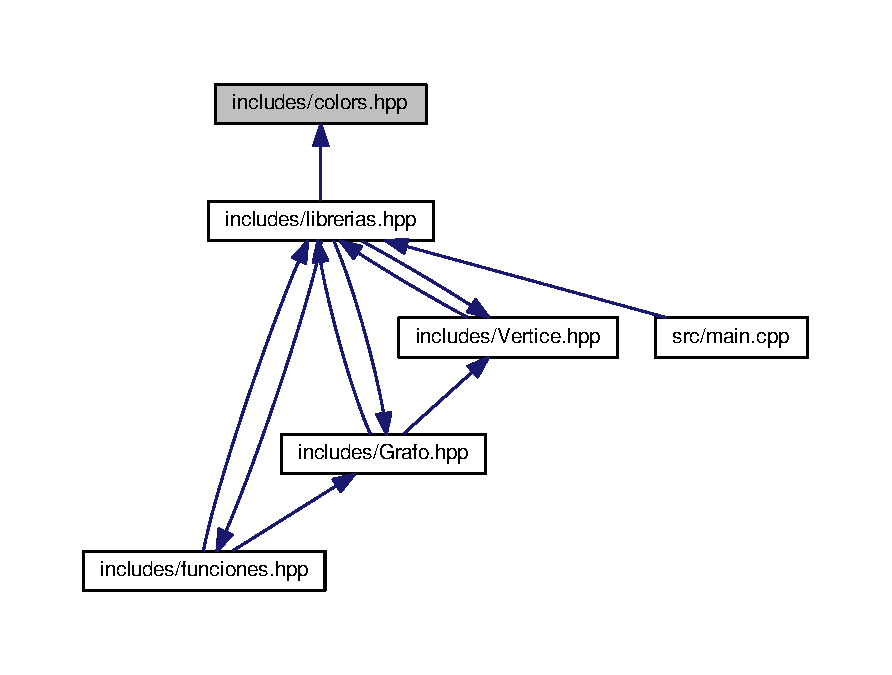
\includegraphics[width=350pt]{colors_8hpp__dep__incl}
\end{center}
\end{figure}
\subsection*{Macros}
\begin{DoxyCompactItemize}
\item 
\#define \hyperlink{colors_8hpp_abb508ea8227673f419e9fe3a86c30d8e}{F\+A\+IL}~\char`\"{}\textbackslash{}033\mbox{[}91m\char`\"{}
\item 
\#define \hyperlink{colors_8hpp_a385c3e1e3d690c32ec87a16e6422d922}{O\+K\+G\+R\+E\+EN}~\char`\"{}\textbackslash{}033\mbox{[}92m\char`\"{}
\item 
\#define \hyperlink{colors_8hpp_a5cb439d9f933fde4cf23caa370c030e7}{W\+A\+R\+N\+I\+NG}~\char`\"{}\textbackslash{}033\mbox{[}93m\char`\"{}
\item 
\#define \hyperlink{colors_8hpp_ad9f51d85a4d6d80cd00f6a3461bb183f}{O\+K\+B\+L\+UE}~\char`\"{}\textbackslash{}033\mbox{[}94m\char`\"{}
\item 
\#define \hyperlink{colors_8hpp_ab7770a7f0d95e67620ff6ed347a07a56}{H\+E\+A\+D\+ER}~\char`\"{}\textbackslash{}033\mbox{[}95m\char`\"{}
\item 
\#define \hyperlink{colors_8hpp_ac9e7df060e19345a81e30a747f8a2d99}{E\+N\+DC}~\char`\"{}\textbackslash{}033\mbox{[}0m\char`\"{}
\end{DoxyCompactItemize}


\subsection{Detailed Description}
Colores para la terminal. 

\begin{DoxyAuthor}{Author}
Jose Manuel Marquez Matarin 
\end{DoxyAuthor}


\subsection{Macro Definition Documentation}
\index{colors.\+hpp@{colors.\+hpp}!E\+N\+DC@{E\+N\+DC}}
\index{E\+N\+DC@{E\+N\+DC}!colors.\+hpp@{colors.\+hpp}}
\subsubsection[{\texorpdfstring{E\+N\+DC}{ENDC}}]{\setlength{\rightskip}{0pt plus 5cm}\#define E\+N\+DC~\char`\"{}\textbackslash{}033\mbox{[}0m\char`\"{}}\hypertarget{colors_8hpp_ac9e7df060e19345a81e30a747f8a2d99}{}\label{colors_8hpp_ac9e7df060e19345a81e30a747f8a2d99}
E\+ND color. \index{colors.\+hpp@{colors.\+hpp}!F\+A\+IL@{F\+A\+IL}}
\index{F\+A\+IL@{F\+A\+IL}!colors.\+hpp@{colors.\+hpp}}
\subsubsection[{\texorpdfstring{F\+A\+IL}{FAIL}}]{\setlength{\rightskip}{0pt plus 5cm}\#define F\+A\+IL~\char`\"{}\textbackslash{}033\mbox{[}91m\char`\"{}}\hypertarget{colors_8hpp_abb508ea8227673f419e9fe3a86c30d8e}{}\label{colors_8hpp_abb508ea8227673f419e9fe3a86c30d8e}
Color red. \index{colors.\+hpp@{colors.\+hpp}!H\+E\+A\+D\+ER@{H\+E\+A\+D\+ER}}
\index{H\+E\+A\+D\+ER@{H\+E\+A\+D\+ER}!colors.\+hpp@{colors.\+hpp}}
\subsubsection[{\texorpdfstring{H\+E\+A\+D\+ER}{HEADER}}]{\setlength{\rightskip}{0pt plus 5cm}\#define H\+E\+A\+D\+ER~\char`\"{}\textbackslash{}033\mbox{[}95m\char`\"{}}\hypertarget{colors_8hpp_ab7770a7f0d95e67620ff6ed347a07a56}{}\label{colors_8hpp_ab7770a7f0d95e67620ff6ed347a07a56}
Color purple. \index{colors.\+hpp@{colors.\+hpp}!O\+K\+B\+L\+UE@{O\+K\+B\+L\+UE}}
\index{O\+K\+B\+L\+UE@{O\+K\+B\+L\+UE}!colors.\+hpp@{colors.\+hpp}}
\subsubsection[{\texorpdfstring{O\+K\+B\+L\+UE}{OKBLUE}}]{\setlength{\rightskip}{0pt plus 5cm}\#define O\+K\+B\+L\+UE~\char`\"{}\textbackslash{}033\mbox{[}94m\char`\"{}}\hypertarget{colors_8hpp_ad9f51d85a4d6d80cd00f6a3461bb183f}{}\label{colors_8hpp_ad9f51d85a4d6d80cd00f6a3461bb183f}
Color blue. \index{colors.\+hpp@{colors.\+hpp}!O\+K\+G\+R\+E\+EN@{O\+K\+G\+R\+E\+EN}}
\index{O\+K\+G\+R\+E\+EN@{O\+K\+G\+R\+E\+EN}!colors.\+hpp@{colors.\+hpp}}
\subsubsection[{\texorpdfstring{O\+K\+G\+R\+E\+EN}{OKGREEN}}]{\setlength{\rightskip}{0pt plus 5cm}\#define O\+K\+G\+R\+E\+EN~\char`\"{}\textbackslash{}033\mbox{[}92m\char`\"{}}\hypertarget{colors_8hpp_a385c3e1e3d690c32ec87a16e6422d922}{}\label{colors_8hpp_a385c3e1e3d690c32ec87a16e6422d922}
Color green. \index{colors.\+hpp@{colors.\+hpp}!W\+A\+R\+N\+I\+NG@{W\+A\+R\+N\+I\+NG}}
\index{W\+A\+R\+N\+I\+NG@{W\+A\+R\+N\+I\+NG}!colors.\+hpp@{colors.\+hpp}}
\subsubsection[{\texorpdfstring{W\+A\+R\+N\+I\+NG}{WARNING}}]{\setlength{\rightskip}{0pt plus 5cm}\#define W\+A\+R\+N\+I\+NG~\char`\"{}\textbackslash{}033\mbox{[}93m\char`\"{}}\hypertarget{colors_8hpp_a5cb439d9f933fde4cf23caa370c030e7}{}\label{colors_8hpp_a5cb439d9f933fde4cf23caa370c030e7}
Color yellow. 
\hypertarget{funciones_8hpp}{}\section{includes/funciones.hpp File Reference}
\label{funciones_8hpp}\index{includes/funciones.\+hpp@{includes/funciones.\+hpp}}


Fichero de funciones que utilizan el grafo.  


{\ttfamily \#include \char`\"{}librerias.\+hpp\char`\"{}}\\*
{\ttfamily \#include \char`\"{}Grafo.\+hpp\char`\"{}}\\*
{\ttfamily \#include $<$iostream$>$}\\*
{\ttfamily \#include $<$string$>$}\\*
{\ttfamily \#include $<$fstream$>$}\\*
{\ttfamily \#include $<$ctype.\+h$>$}\\*
Include dependency graph for funciones.\+hpp\+:\nopagebreak
\begin{figure}[H]
\begin{center}
\leavevmode
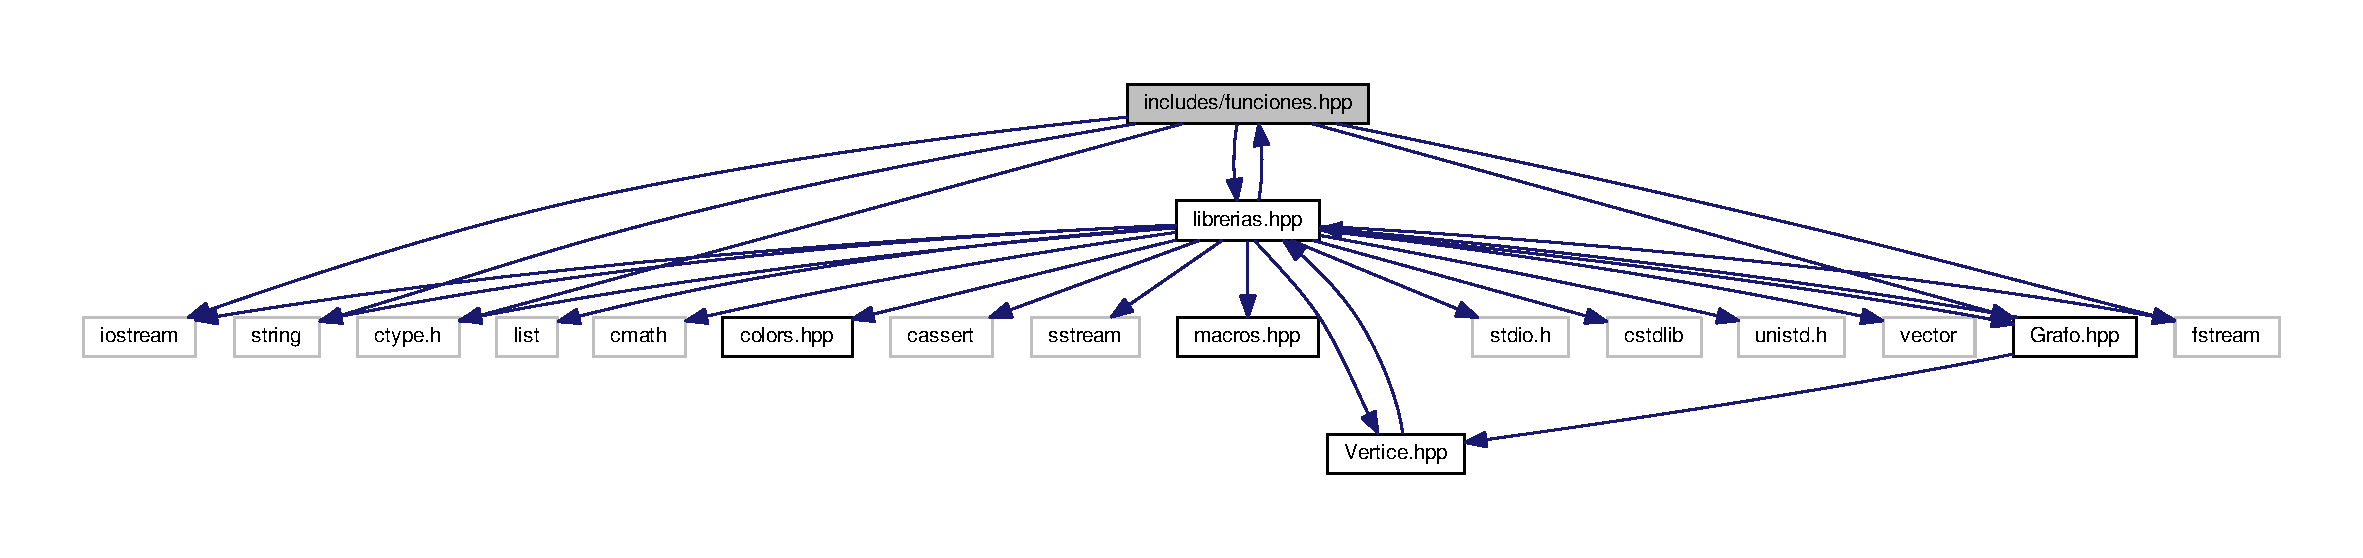
\includegraphics[width=350pt]{funciones_8hpp__incl}
\end{center}
\end{figure}
This graph shows which files directly or indirectly include this file\+:\nopagebreak
\begin{figure}[H]
\begin{center}
\leavevmode
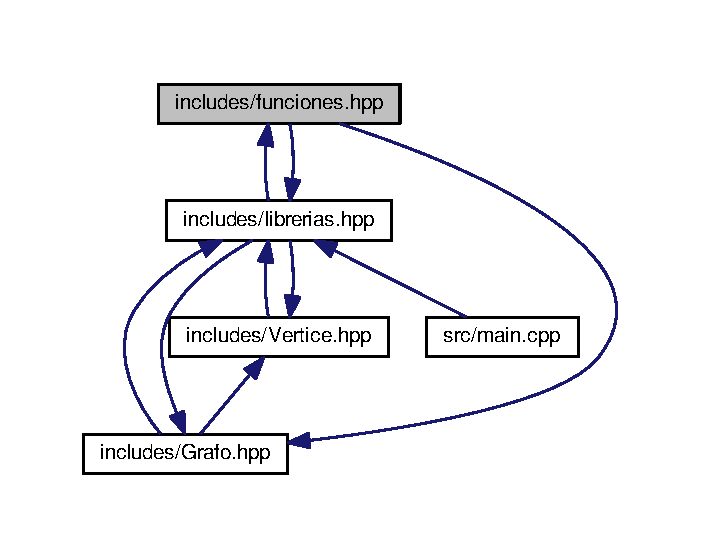
\includegraphics[width=337pt]{funciones_8hpp__dep__incl}
\end{center}
\end{figure}
\subsection*{Namespaces}
\begin{DoxyCompactItemize}
\item 
 \hyperlink{namespaceed}{ed}
\begin{DoxyCompactList}\small\item\em Espacio de nombres ed. \end{DoxyCompactList}\end{DoxyCompactItemize}
\subsection*{Functions}
\begin{DoxyCompactItemize}
\item 
Grafo $\ast$ \hyperlink{namespaceed_a564e754c90ffdcd64910fad4d2e3a2bf}{ed\+::cargar\+Fichero} (std\+::string file\+\_\+name)
\begin{DoxyCompactList}\small\item\em Funcion para cargar el grafo desde un fichero pasado por parametro. \end{DoxyCompactList}\item 
void \hyperlink{namespaceed_adccb5659f086f7308fc2a87653ae5490}{ed\+::mostrar\+Grafo} (Grafo $\ast$grafo)
\begin{DoxyCompactList}\small\item\em Funcion que muestra el grafo por pantalla. \end{DoxyCompactList}\item 
void \hyperlink{namespaceed_a5f0ef37f4003571c0d06cd5ed1113939}{ed\+::camino\+Minimo} (Grafo $\ast$grafo, int $\ast$$\ast$matriz\+\_\+recorridos, Vertice \&origen, Vertice \&destino)
\begin{DoxyCompactList}\small\item\em Funcion que calcula el camino minimo entre dos vertices. \end{DoxyCompactList}\item 
int \hyperlink{namespaceed_a6d0e98c85a44d58e0cc6560de8dc51d1}{ed\+::\+Suma\+Distancias} (Grafo $\ast$grafo, double $\ast$$\ast$matriz\+\_\+distancias, Vertice v)
\begin{DoxyCompactList}\small\item\em Funcion que muestra la suma de distancias a cada vertice tomando como origen el vertice pasado por parametro. \end{DoxyCompactList}\item 
void \hyperlink{namespaceed_a81f41376971c7b12ebf614903df91cd2}{ed\+::\+Vertice\+Menor\+Suma} (Grafo $\ast$grafo, double $\ast$$\ast$matriz\+\_\+distancias)
\begin{DoxyCompactList}\small\item\em Funcion que muestra el vertice cuya suma de distancias es menor. \end{DoxyCompactList}\item 
void \hyperlink{namespaceed_af547530c0f015ed298c59837343a9b5e}{ed\+::algoritmo\+\_\+floyd} (Grafo $\ast$\&grafo, double $\ast$$\ast$\&matriz\+\_\+distancias, int $\ast$$\ast$\&matriz\+\_\+recorridos)
\begin{DoxyCompactList}\small\item\em Funcion que aplica el algoritmo de floyd al grafo pasado por parametro. \end{DoxyCompactList}\end{DoxyCompactItemize}


\subsection{Detailed Description}
Fichero de funciones que utilizan el grafo. 

\begin{DoxyAuthor}{Author}
Jose Manuel Marquez Matarin 
\end{DoxyAuthor}

\hypertarget{Grafo_8hpp}{}\section{includes/\+Grafo.hpp File Reference}
\label{Grafo_8hpp}\index{includes/\+Grafo.\+hpp@{includes/\+Grafo.\+hpp}}


Clase Grafo.  


{\ttfamily \#include \char`\"{}librerias.\+hpp\char`\"{}}\\*
{\ttfamily \#include \char`\"{}Vertice.\+hpp\char`\"{}}\\*
Include dependency graph for Grafo.\+hpp\+:\nopagebreak
\begin{figure}[H]
\begin{center}
\leavevmode
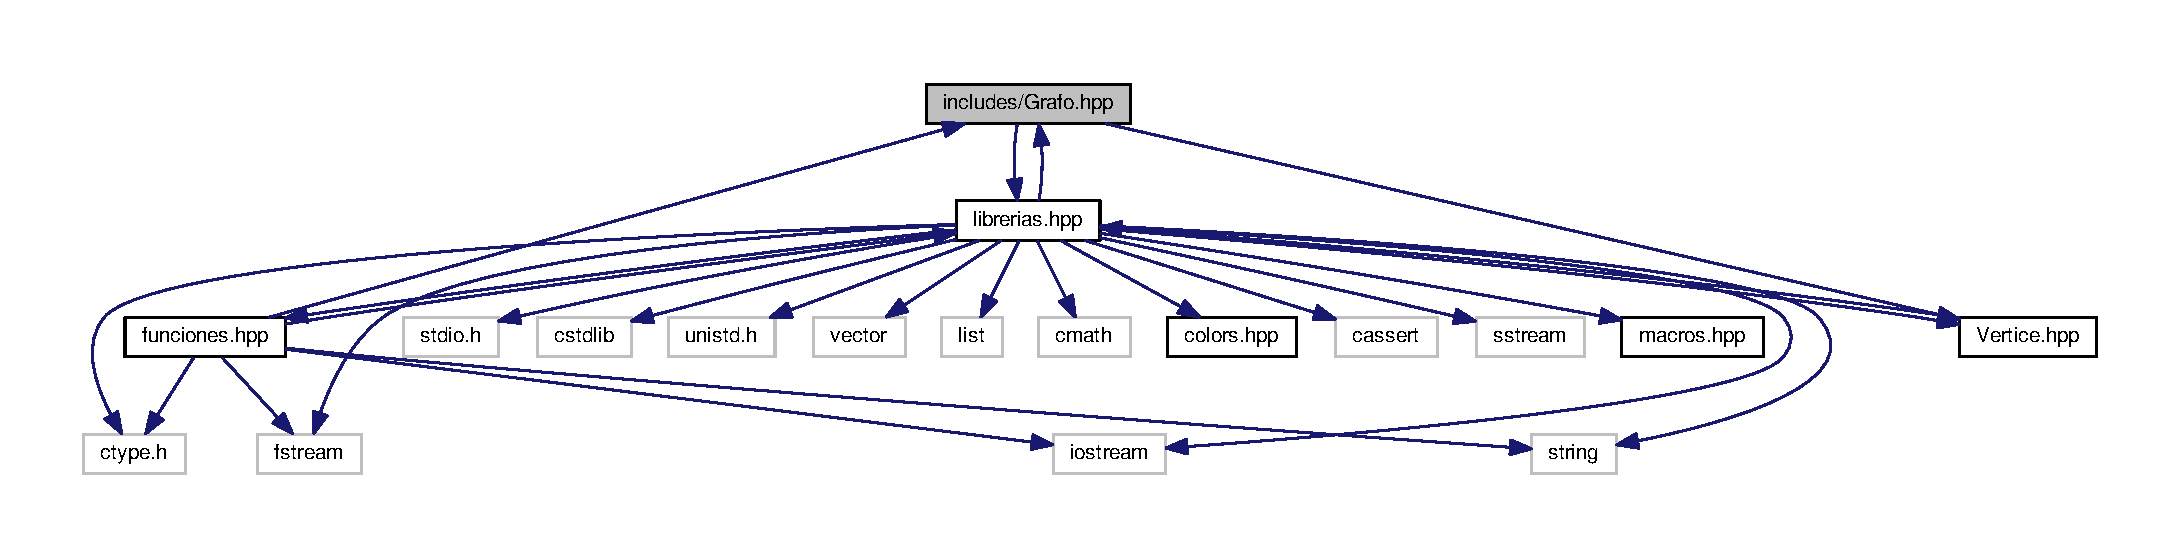
\includegraphics[width=350pt]{Grafo_8hpp__incl}
\end{center}
\end{figure}
This graph shows which files directly or indirectly include this file\+:\nopagebreak
\begin{figure}[H]
\begin{center}
\leavevmode
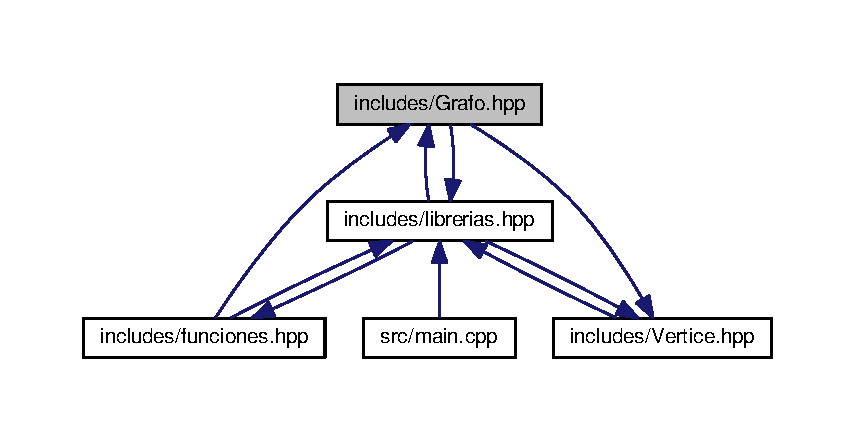
\includegraphics[width=350pt]{Grafo_8hpp__dep__incl}
\end{center}
\end{figure}
\subsection*{Classes}
\begin{DoxyCompactItemize}
\item 
class \hyperlink{classed_1_1Grafo}{ed\+::\+Grafo}
\end{DoxyCompactItemize}
\subsection*{Namespaces}
\begin{DoxyCompactItemize}
\item 
 \hyperlink{namespaceed}{ed}
\begin{DoxyCompactList}\small\item\em Espacio de nombres ed. \end{DoxyCompactList}\end{DoxyCompactItemize}
\subsection*{Macros}
\begin{DoxyCompactItemize}
\item 
\#define \hyperlink{Grafo_8hpp_af076440f216f5a40a11563e489f04932}{I\+N\+F\+I\+N\+I\+TO}~999999
\end{DoxyCompactItemize}


\subsection{Detailed Description}
Clase Grafo. 

\begin{DoxyAuthor}{Author}
Jose Manuel Marquez Matarin 
\end{DoxyAuthor}


\subsection{Macro Definition Documentation}
\index{Grafo.\+hpp@{Grafo.\+hpp}!I\+N\+F\+I\+N\+I\+TO@{I\+N\+F\+I\+N\+I\+TO}}
\index{I\+N\+F\+I\+N\+I\+TO@{I\+N\+F\+I\+N\+I\+TO}!Grafo.\+hpp@{Grafo.\+hpp}}
\subsubsection[{\texorpdfstring{I\+N\+F\+I\+N\+I\+TO}{INFINITO}}]{\setlength{\rightskip}{0pt plus 5cm}\#define I\+N\+F\+I\+N\+I\+TO~999999}\hypertarget{Grafo_8hpp_af076440f216f5a40a11563e489f04932}{}\label{Grafo_8hpp_af076440f216f5a40a11563e489f04932}
Valor de I\+N\+F\+I\+N\+I\+TO. 
\hypertarget{librerias_8hpp}{}\section{includes/librerias.hpp File Reference}
\label{librerias_8hpp}\index{includes/librerias.\+hpp@{includes/librerias.\+hpp}}


Librerias incluidas en los hpp.  


{\ttfamily \#include $<$iostream$>$}\\*
{\ttfamily \#include $<$stdio.\+h$>$}\\*
{\ttfamily \#include $<$cstdlib$>$}\\*
{\ttfamily \#include $<$unistd.\+h$>$}\\*
{\ttfamily \#include $<$string$>$}\\*
{\ttfamily \#include $<$vector$>$}\\*
{\ttfamily \#include $<$list$>$}\\*
{\ttfamily \#include $<$ctype.\+h$>$}\\*
{\ttfamily \#include $<$cmath$>$}\\*
{\ttfamily \#include \char`\"{}colors.\+hpp\char`\"{}}\\*
{\ttfamily \#include $<$fstream$>$}\\*
{\ttfamily \#include $<$cassert$>$}\\*
{\ttfamily \#include $<$sstream$>$}\\*
{\ttfamily \#include \char`\"{}macros.\+hpp\char`\"{}}\\*
{\ttfamily \#include \char`\"{}Donante.\+hpp\char`\"{}}\\*
{\ttfamily \#include \char`\"{}Donantes\+Interfaz.\+hpp\char`\"{}}\\*
{\ttfamily \#include \char`\"{}Donante\+Interfaz.\+hpp\char`\"{}}\\*
{\ttfamily \#include \char`\"{}Monticulo\+Interfaz.\+hpp\char`\"{}}\\*
{\ttfamily \#include \char`\"{}Monticulo.\+hpp\char`\"{}}\\*
Include dependency graph for librerias.\+hpp\+:
\nopagebreak
\begin{figure}[H]
\begin{center}
\leavevmode
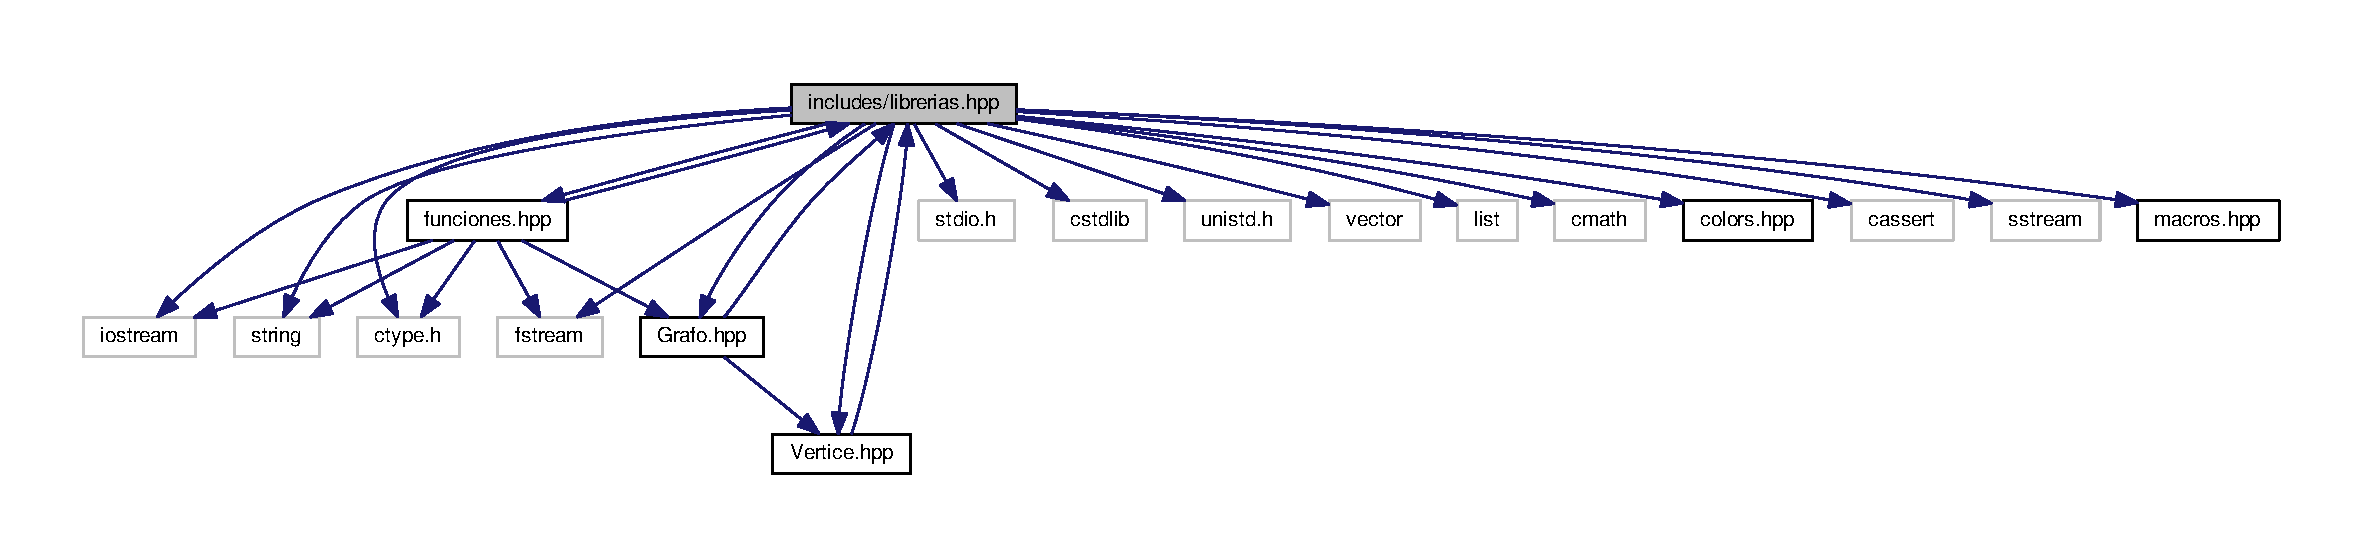
\includegraphics[width=350pt]{librerias_8hpp__incl}
\end{center}
\end{figure}
This graph shows which files directly or indirectly include this file\+:
\nopagebreak
\begin{figure}[H]
\begin{center}
\leavevmode
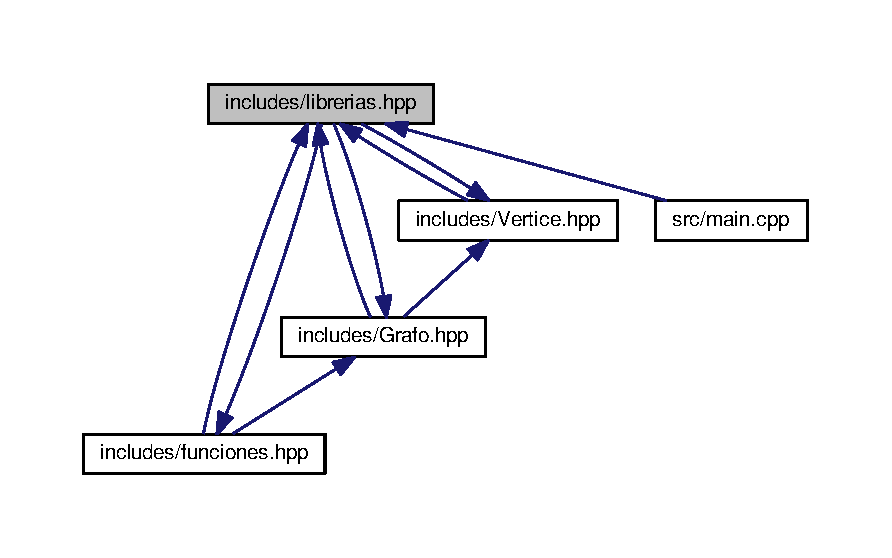
\includegraphics[width=350pt]{librerias_8hpp__dep__incl}
\end{center}
\end{figure}


\subsection{Detailed Description}
Librerias incluidas en los hpp. 

\begin{DoxyAuthor}{Author}
Jose Manuel Marquez Matarin 
\end{DoxyAuthor}

\hypertarget{macros_8hpp}{}\section{includes/macros.hpp File Reference}
\label{macros_8hpp}\index{includes/macros.\+hpp@{includes/macros.\+hpp}}


Macros para el diseño de pantallas.  


This graph shows which files directly or indirectly include this file\+:
\nopagebreak
\begin{figure}[H]
\begin{center}
\leavevmode
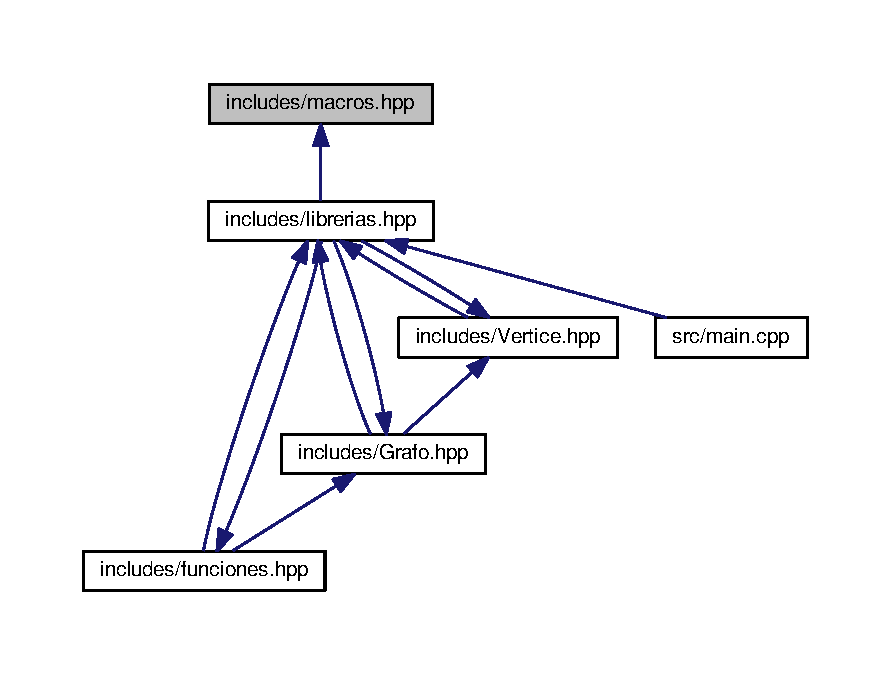
\includegraphics[width=350pt]{macros_8hpp__dep__incl}
\end{center}
\end{figure}
\subsection*{Macros}
\begin{DoxyCompactItemize}
\item 
\#define \hyperlink{macros_8hpp_a1e26748f72802cc32341cc3846db931f}{L\+U\+G\+AR}(x,  y)~printf(\char`\"{}\textbackslash{}033\mbox{[}\%d;\%dH\char`\"{}, x, y)
\item 
\#define \hyperlink{macros_8hpp_a79bf316fce01e63d76dddcdcbe72ab1c}{B\+O\+R\+R\+AR}~printf(\char`\"{}\textbackslash{}33\mbox{[}2\+J\char`\"{})
\item 
\#define \hyperlink{macros_8hpp_ab86c2fc65d2b4c5205910f548828dcb9}{P\+A\+R\+P\+A\+D\+EO}~printf(\char`\"{}\%c\mbox{[}5m\char`\"{}, 27)
\item 
\#define \hyperlink{macros_8hpp_af2815fb445b50124864e3f2f958fac24}{A\+P\+A\+GA}~printf(\char`\"{}\%c\mbox{[}0m\char`\"{}, 27)
\item 
\#define \hyperlink{macros_8hpp_ac6cb5eae7b643f5d13c9d546e81dbcaf}{I\+N\+V\+E\+R\+SO}~printf(\char`\"{}\%c\mbox{[}7m\char`\"{}, 27)
\item 
\#define \hyperlink{macros_8hpp_a3ab8b4157fd29a2336c702b26a967bb9}{S\+U\+B\+R\+A\+Y\+A\+DO}~printf(\char`\"{}\%c\mbox{[}4m\char`\"{}, 27)
\item 
\#define \hyperlink{macros_8hpp_af7eea73aeb56d77e1d56471ab214f8e2}{I\+N\+T\+E\+N\+S\+I\+D\+AD}~printf(\char`\"{}\%c\mbox{[}1m\char`\"{}, 27)
\end{DoxyCompactItemize}


\subsection{Detailed Description}
Macros para el diseño de pantallas. 



\subsection{Macro Definition Documentation}
\index{macros.\+hpp@{macros.\+hpp}!A\+P\+A\+GA@{A\+P\+A\+GA}}
\index{A\+P\+A\+GA@{A\+P\+A\+GA}!macros.\+hpp@{macros.\+hpp}}
\subsubsection[{\texorpdfstring{A\+P\+A\+GA}{APAGA}}]{\setlength{\rightskip}{0pt plus 5cm}\#define A\+P\+A\+GA~printf(\char`\"{}\%c\mbox{[}0m\char`\"{}, 27)}\hypertarget{macros_8hpp_af2815fb445b50124864e3f2f958fac24}{}\label{macros_8hpp_af2815fb445b50124864e3f2f958fac24}
Macro of interaction. \index{macros.\+hpp@{macros.\+hpp}!B\+O\+R\+R\+AR@{B\+O\+R\+R\+AR}}
\index{B\+O\+R\+R\+AR@{B\+O\+R\+R\+AR}!macros.\+hpp@{macros.\+hpp}}
\subsubsection[{\texorpdfstring{B\+O\+R\+R\+AR}{BORRAR}}]{\setlength{\rightskip}{0pt plus 5cm}\#define B\+O\+R\+R\+AR~printf(\char`\"{}\textbackslash{}33\mbox{[}2\+J\char`\"{})}\hypertarget{macros_8hpp_a79bf316fce01e63d76dddcdcbe72ab1c}{}\label{macros_8hpp_a79bf316fce01e63d76dddcdcbe72ab1c}
Macro for delete. \index{macros.\+hpp@{macros.\+hpp}!I\+N\+T\+E\+N\+S\+I\+D\+AD@{I\+N\+T\+E\+N\+S\+I\+D\+AD}}
\index{I\+N\+T\+E\+N\+S\+I\+D\+AD@{I\+N\+T\+E\+N\+S\+I\+D\+AD}!macros.\+hpp@{macros.\+hpp}}
\subsubsection[{\texorpdfstring{I\+N\+T\+E\+N\+S\+I\+D\+AD}{INTENSIDAD}}]{\setlength{\rightskip}{0pt plus 5cm}\#define I\+N\+T\+E\+N\+S\+I\+D\+AD~printf(\char`\"{}\%c\mbox{[}1m\char`\"{}, 27)}\hypertarget{macros_8hpp_af7eea73aeb56d77e1d56471ab214f8e2}{}\label{macros_8hpp_af7eea73aeb56d77e1d56471ab214f8e2}
Macro of interaction. \index{macros.\+hpp@{macros.\+hpp}!I\+N\+V\+E\+R\+SO@{I\+N\+V\+E\+R\+SO}}
\index{I\+N\+V\+E\+R\+SO@{I\+N\+V\+E\+R\+SO}!macros.\+hpp@{macros.\+hpp}}
\subsubsection[{\texorpdfstring{I\+N\+V\+E\+R\+SO}{INVERSO}}]{\setlength{\rightskip}{0pt plus 5cm}\#define I\+N\+V\+E\+R\+SO~printf(\char`\"{}\%c\mbox{[}7m\char`\"{}, 27)}\hypertarget{macros_8hpp_ac6cb5eae7b643f5d13c9d546e81dbcaf}{}\label{macros_8hpp_ac6cb5eae7b643f5d13c9d546e81dbcaf}
Macro of interaction. \index{macros.\+hpp@{macros.\+hpp}!L\+U\+G\+AR@{L\+U\+G\+AR}}
\index{L\+U\+G\+AR@{L\+U\+G\+AR}!macros.\+hpp@{macros.\+hpp}}
\subsubsection[{\texorpdfstring{L\+U\+G\+AR}{LUGAR}}]{\setlength{\rightskip}{0pt plus 5cm}\#define L\+U\+G\+AR(
\begin{DoxyParamCaption}
\item[{}]{x, }
\item[{}]{y}
\end{DoxyParamCaption}
)~printf(\char`\"{}\textbackslash{}033\mbox{[}\%d;\%dH\char`\"{}, x, y)}\hypertarget{macros_8hpp_a1e26748f72802cc32341cc3846db931f}{}\label{macros_8hpp_a1e26748f72802cc32341cc3846db931f}
Macro for place. \index{macros.\+hpp@{macros.\+hpp}!P\+A\+R\+P\+A\+D\+EO@{P\+A\+R\+P\+A\+D\+EO}}
\index{P\+A\+R\+P\+A\+D\+EO@{P\+A\+R\+P\+A\+D\+EO}!macros.\+hpp@{macros.\+hpp}}
\subsubsection[{\texorpdfstring{P\+A\+R\+P\+A\+D\+EO}{PARPADEO}}]{\setlength{\rightskip}{0pt plus 5cm}\#define P\+A\+R\+P\+A\+D\+EO~printf(\char`\"{}\%c\mbox{[}5m\char`\"{}, 27)}\hypertarget{macros_8hpp_ab86c2fc65d2b4c5205910f548828dcb9}{}\label{macros_8hpp_ab86c2fc65d2b4c5205910f548828dcb9}
Macro of interaction. \index{macros.\+hpp@{macros.\+hpp}!S\+U\+B\+R\+A\+Y\+A\+DO@{S\+U\+B\+R\+A\+Y\+A\+DO}}
\index{S\+U\+B\+R\+A\+Y\+A\+DO@{S\+U\+B\+R\+A\+Y\+A\+DO}!macros.\+hpp@{macros.\+hpp}}
\subsubsection[{\texorpdfstring{S\+U\+B\+R\+A\+Y\+A\+DO}{SUBRAYADO}}]{\setlength{\rightskip}{0pt plus 5cm}\#define S\+U\+B\+R\+A\+Y\+A\+DO~printf(\char`\"{}\%c\mbox{[}4m\char`\"{}, 27)}\hypertarget{macros_8hpp_a3ab8b4157fd29a2336c702b26a967bb9}{}\label{macros_8hpp_a3ab8b4157fd29a2336c702b26a967bb9}
Macro of interaction. 
\hypertarget{Vertice_8hpp}{}\section{includes/\+Vertice.hpp File Reference}
\label{Vertice_8hpp}\index{includes/\+Vertice.\+hpp@{includes/\+Vertice.\+hpp}}


Clase Vertice.  


{\ttfamily \#include \char`\"{}librerias.\+hpp\char`\"{}}\\*
Include dependency graph for Vertice.\+hpp\+:\nopagebreak
\begin{figure}[H]
\begin{center}
\leavevmode
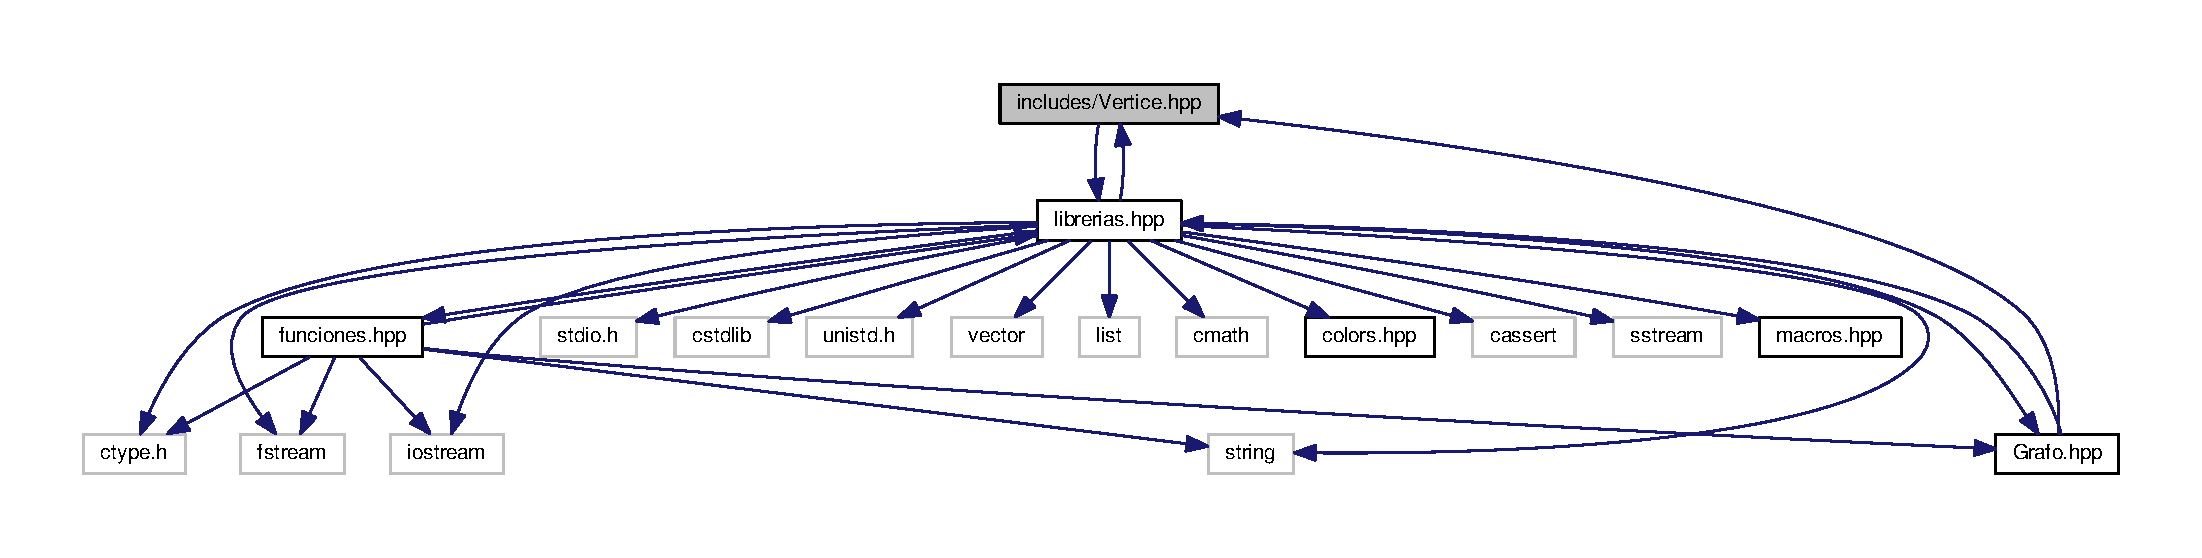
\includegraphics[width=350pt]{Vertice_8hpp__incl}
\end{center}
\end{figure}
This graph shows which files directly or indirectly include this file\+:\nopagebreak
\begin{figure}[H]
\begin{center}
\leavevmode
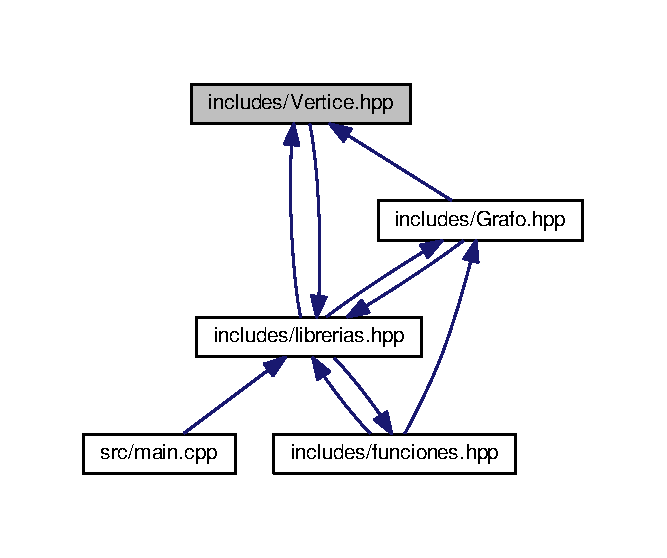
\includegraphics[width=320pt]{Vertice_8hpp__dep__incl}
\end{center}
\end{figure}
\subsection*{Classes}
\begin{DoxyCompactItemize}
\item 
class \hyperlink{classed_1_1Vertice}{ed\+::\+Vertice}
\end{DoxyCompactItemize}
\subsection*{Namespaces}
\begin{DoxyCompactItemize}
\item 
 \hyperlink{namespaceed}{ed}
\begin{DoxyCompactList}\small\item\em Espacio de nombres ed. \end{DoxyCompactList}\end{DoxyCompactItemize}


\subsection{Detailed Description}
Clase Vertice. 

\begin{DoxyAuthor}{Author}
Jose Manuel Marquez Matarin 
\end{DoxyAuthor}

\hypertarget{main_8cpp}{}\section{src/main.cpp File Reference}
\label{main_8cpp}\index{src/main.\+cpp@{src/main.\+cpp}}


Main monomio.  


{\ttfamily \#include \char`\"{}../includes/librerias.\+hpp\char`\"{}}\\*
Include dependency graph for main.\+cpp\+:
% FIG 0
\subsection*{Functions}
\begin{DoxyCompactItemize}
\item 
\hypertarget{main_8cpp_ae66f6b31b5ad750f1fe042a706a4e3d4}{}int {\bfseries main} ()\label{main_8cpp_ae66f6b31b5ad750f1fe042a706a4e3d4}

\end{DoxyCompactItemize}


\subsection{Detailed Description}
Main monomio. 

\begin{DoxyAuthor}{Author}
Jose M. Márquez Matarín 
\end{DoxyAuthor}

%--- End generated contents ---

% Index
\backmatter
\newpage
\phantomsection
\clearemptydoublepage
\addcontentsline{toc}{chapter}{Index}
\printindex

\end{document}
